\subsection{Boucles de détections évenementielles}

Deux évenements critiques de la mission sont détectés électroniquement par le système embarqué : le décollage et la séparation
inter-étage.\\

% \hspace*{-\parindent}%
% \begin{minipage}{0.44\textwidth}
%     Chaque séquenceur possède deux connecteurs deux pins composés d'un signal d'entrée configuré en pull-up et d'une masse. En
%     formant un circuit entre ces deux pins, deux états sont possibles : un circuit fermé ou un circuit ouvert.
%     \begin{itemize}
%         \item Circuit fermé : le signal est connecté à la masse en basse impédance.
%         \item Circuit ouvert : le signal est connecté à la tension d'alimentation en haute
%         impédance.
%     \end{itemize}

%     \noindent Jouer sur l'état du circuit permet de détecter ces événements critiques. Un code couleur a été utilisé afin de
%     faciliter l'identification: le vert pour la détection du \textcolor{green}{décollage} et le bleu pour la détection de la
%     \textcolor{blue}{séparation inter-étage}. Le schéma de principe de ces boucles de détection avec l'utilisation de la carte
%     routage est présenté à la figure \ref{fig:systeme_jack_sepa} ci-dessous.
% \end{minipage}
% \hfill
% \begin{minipage}{0.55\textwidth}
%     \centering
%     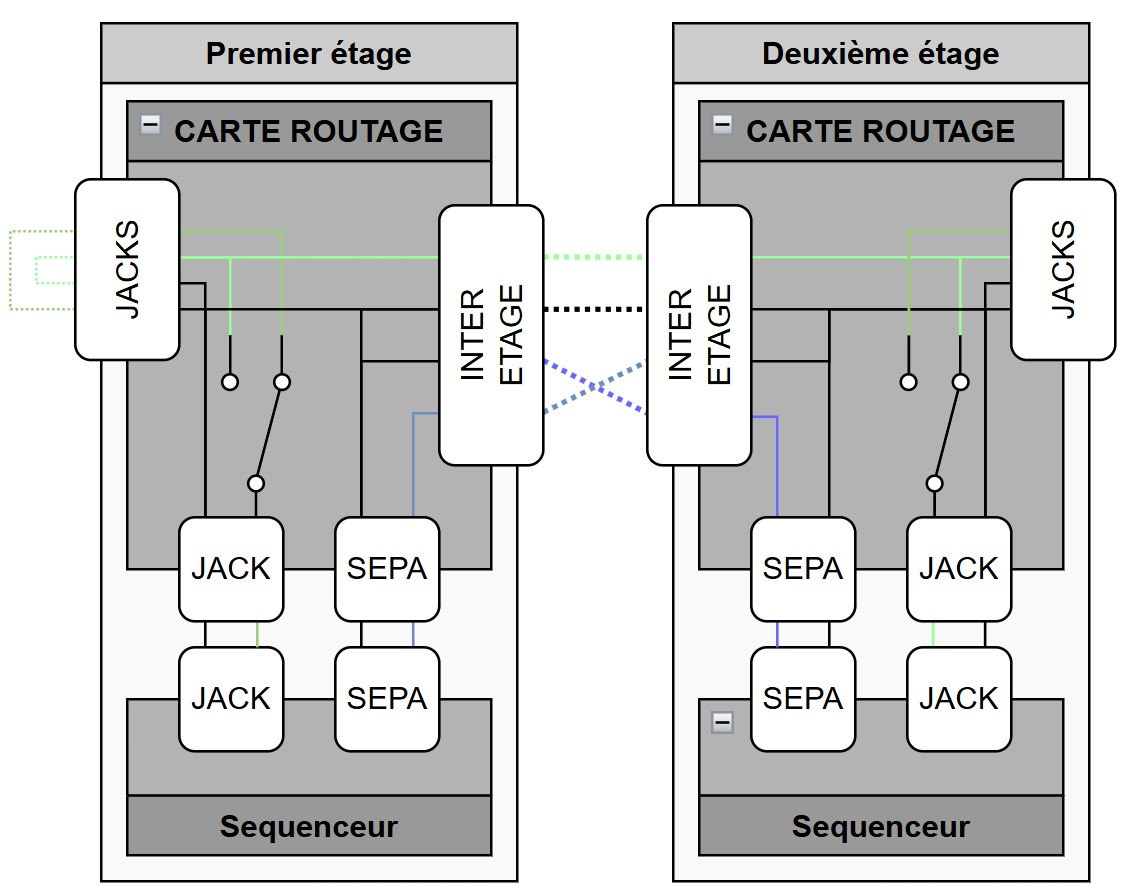
\includegraphics[width=\textwidth]{figures/elec/systeme_jack_sepa.jpg}
%     \captionof{figure}{Système de détection du décollage et de la séparation inter-étage}
%     \label{fig:systeme_jack_sepa}
% \end{minipage}

% \vspace{0.5cm}

Chaque séquenceur possède deux connecteurs deux pins composés d'un signal d'entrée configuré en pull-up et d'une masse. En formant
un circuit entre ces deux pins, deux états sont possibles : un circuit fermé ou un circuit ouvert.
\begin{itemize}
    \item Circuit fermé : le signal est connecté à la masse en basse impédance.
    \item Circuit ouvert : le signal est connecté à la tension d'alimentation en haute
    impédance.
\end{itemize}

\noindent Jouer sur l'état du circuit permet de détecter ces événements critiques. Un code couleur a été utilisé afin de faciliter
l'identification: le vert pour la détection du \textcolor{green}{décollage}, le bleu pour la détection de la
\textcolor{blue}{séparation inter-étage} et le noir pour la masse. Le schéma de principe de ces boucles de détection avec
l'utilisation de la carte routage est présenté à la figure \ref{fig:systeme_jack_sepa} ci-dessous.

\begin{figure}[H]
    \centering
    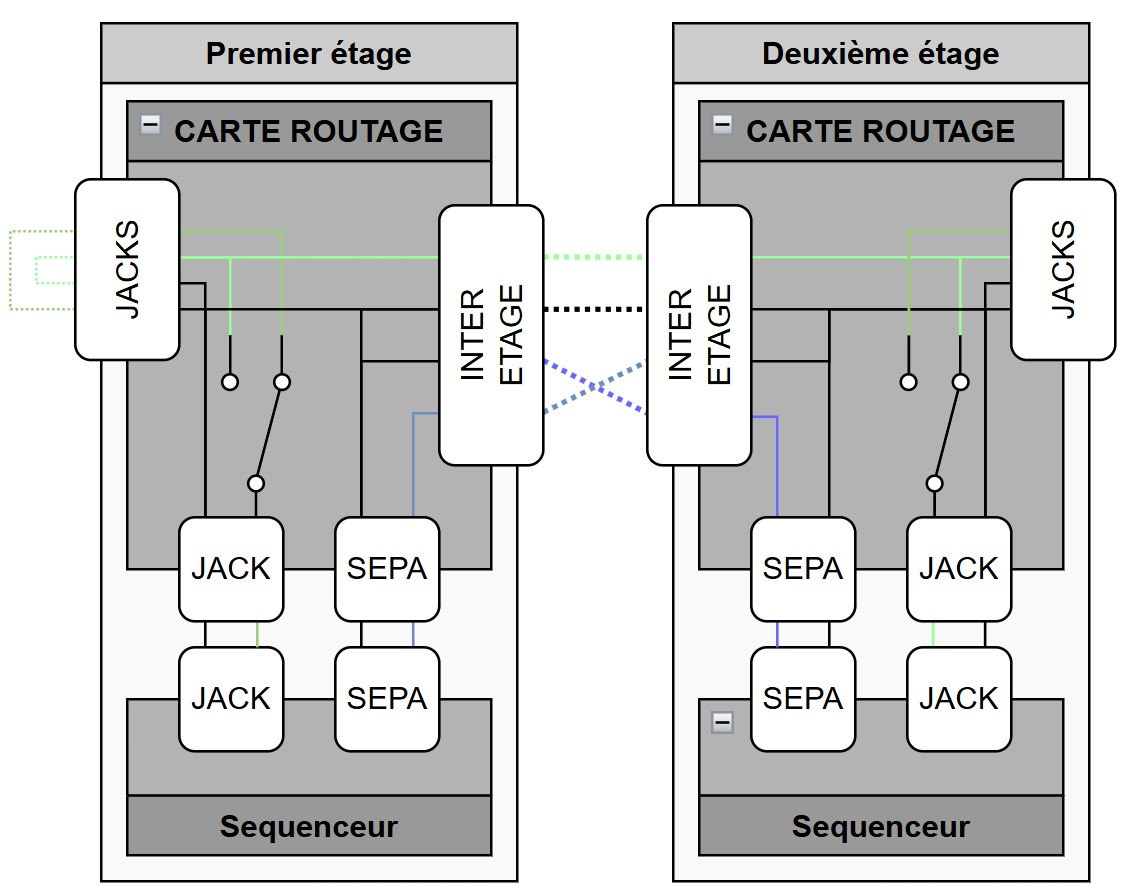
\includegraphics[width=0.8\textwidth]{figures/elec/systeme_jack_sepa.jpg}
    \caption{Système de détection du décollage et de la séparation inter-étage}
    \label{fig:systeme_jack_sepa}
\end{figure}

Les cartes de routage sont les mêmes sur le premier et le deuxième étage. La seule différence est la configuration du connecteur
\verb|JACK| branché au séquenceur. Schématisé sur la figure plus haut par un interupteur, la carte possède deux empruntes de
résistance zéro ohm permettant de choisir entre deux configurations : une pour le premier étage et une pour le deuxième étage. En
effet nous voulons que chaque étage ait sa propre boucle de détection du décollage et de la séparation inter-étage.\\

Il y a donc 4 signaux distincts : \verb|jack_1| et \verb|sepa_1| pour le premier étage et \verb|jack_2| et \verb|sepa_2| pour le
deuxième étage. \verb|sepa_1| et \verb|sepa_2| ne se retrouvent jamais sur une même carte l'électronique au vu de la symétrie du
système ce qui n'est pas le cas pour \verb|jack_1| et \verb|jack_2| bien ne sont pas connectés entre eux. La boucle du signal
\verb|jack_1| n'est branchée qu'au connecteur nommé \verb|JACKS| tandis que celle du signal \verb|jack_2| l'est également au
connecteur \verb|INTER ETAGE| lui permettant de traverser les deux étages. Ainsi :\\

\begin{itemize}
    \item Pour le premier étage, le signal \verb|jack_1| part du séquenceur du premier étage, arrive sur la carte de routage du
    premier étage au travers du connecteur \verb|JACK|, sort de la carte par le connecteur \verb|JACKS| où la boucle est formée.
    \item Pour le deuxième étage, le signal \verb|jack_2| part du séquenceur du deuxième étage, arrive sur la carte de routage du
    deuxième étage au travers du connecteur \verb|JACK|, sort de la carte par le connecteur \verb|INTER ETAGE|, rentre dans la carte
    routage du premier étage et enfin sort de cette dernière par le connecteur \verb|JACKS| où la boucle est formée.
\end{itemize}


Le connecteur \verb|INTER ETAGE| schématisé sur la figure \ref{fig:connexion_inter_etage} représente en réalité un ensemble de
4 connecteurs JST 3 pins offrant un total de 12 broches. Ces 12 broches sont réparties sur 2 connecteurs de bord de carte, les
connecteurs se trouvant sur le deuxième étage et les cartes rentrant dans ces connecteurs, sur le premier étage et monté dans
directement dans le système de séparation. 4 signaux doivent passer par ce connecteur : \verb|jack_2|, \verb|sepa_1|,
\verb|sepa_2| et la masse. Avec 12 broche, il est alors possible d'obtenir une redondance de 3 broches par signaux afin d'assurer
la continuité du signal même en cas de défaillance d'une broche ou de mauvais contact.

\vspace{0.5cm}

\hspace*{-\parindent}%
\begin{minipage}{0.40\textwidth}
    \centering
    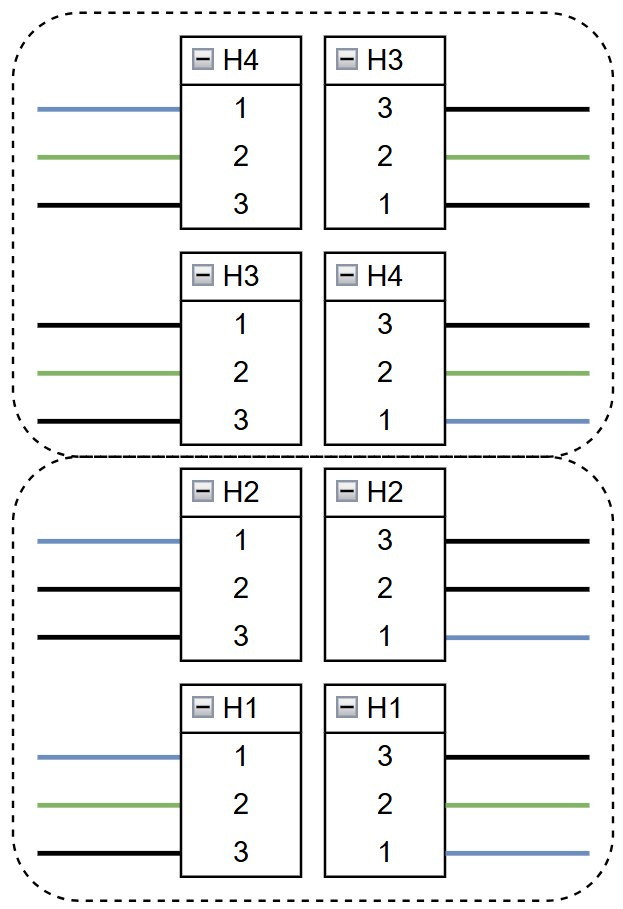
\includegraphics[width=\textwidth]{figures/elec/connexion_inter_etage.jpg}
    \captionof{figure}{Schéma de la connexion inter-étage}
    \label{fig:connexion_inter_etage}
\end{minipage}
\hfill
\begin{minipage}{0.18\textwidth}
    \centering
    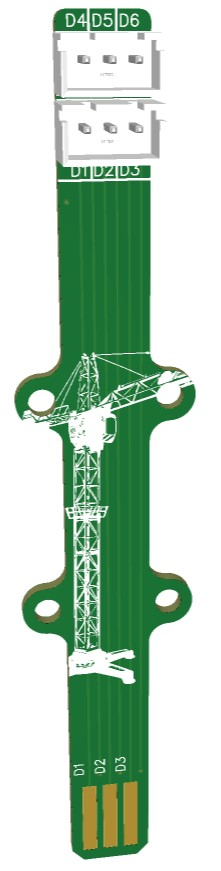
\includegraphics[width=0.8\textwidth]{figures/elec/PCB_connexion_sepa.jpg}
    \captionof{figure}{PCB de la connexion inter-étage}
\end{minipage}
\hfill
\begin{minipage}{0.30\textwidth}
    Nous avons créer une nomencalture pour les 4 jst sortant de la carte routage
    des étages : \verb|H1|, \verb|H2|, \verb|H3| et \verb|H4| et établie une règle de connexion pin à pin de ces connecteurs.
    Ainsi nous avons :
    \begin{itemize}
        \item \verb|H1| $\Longleftrightarrow$ \verb|H1|
        \item \verb|H2| $\Longleftrightarrow$ \verb|H2|
        \item \verb|H3| $\Longleftrightarrow$ \verb|H4|
        \item \verb|H4| $\Longleftrightarrow$ \verb|H3|
    \end{itemize}
    Avec également la règle de connexion pin à pin suivante :
    \begin{itemize}
        \item Pin 1 $\Longleftrightarrow$ Pin 3
        \item Pin 2 $\Longleftrightarrow$ Pin 2
        \item Pin 3 $\Longleftrightarrow$ Pin 1
    \end{itemize}

    Aussi, les jsts \verb|H1| et \verb|H2| sont regroupés sur le même connecteur de bord de carte et les jsts \verb|H3| et
    \verb|H4| sur l'autre connecteur de bord de carte.\\

    Toutes ces règles de connexion peuvent être visualisées sur la figure \ref{fig:connexion_inter_etage} ci-contre.\\
\end{minipage}

\vfill

\begin{figure}[h]
    \centering
    \begin{subfigure}{0.45\textwidth}
        \centering
        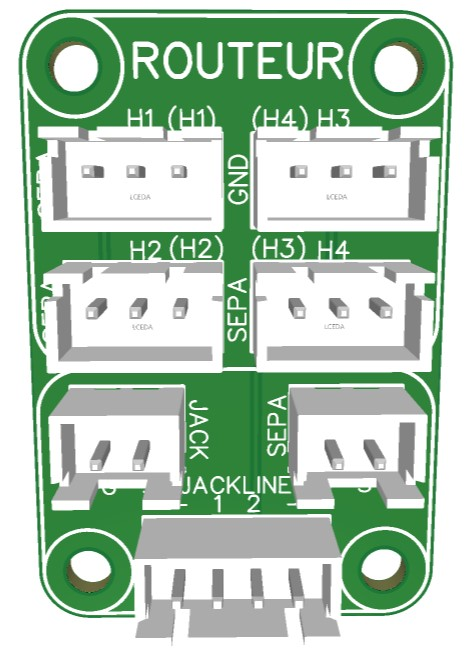
\includegraphics[width=0.55\textwidth]{figures/elec/PCB_routeur.jpg}
        \caption{PCB de routage du système de détection du décollage et de la séparation inter-étage}
        \label{fig:PCB_routeur}
    \end{subfigure}
    \hfill
    \begin{subfigure}{0.45\textwidth}
        \centering
        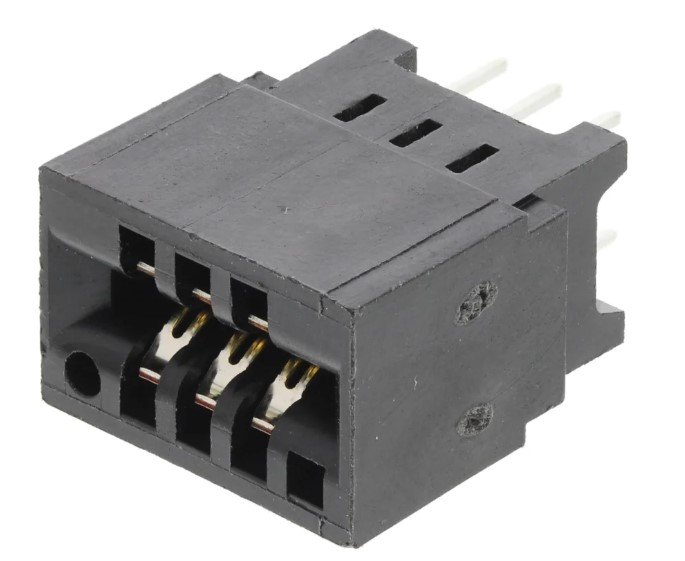
\includegraphics[width=0.8\textwidth]{figures/elec/pcb_edge_connector.jpg}
        \caption{Connecteur de bord de carte se trouvant sur la partie du système de séparation du deuxième étage}
        \label{fig:PCB_connexion_sepa}
    \end{subfigure}
    \caption{PCB routage et connecteur de bord de PCB}
\end{figure}

\vfill

\newpage
